\chapter{Work Done}

\section{Work Done}

\subsection{Pieces}
\paragraph{}
The pieces extensively use the concept of inheritance and Abstraction. There is a an abstract Piece class which is inherited by all the 6 pieces: Pawn, Rook, Knight, Bishop, Queen and King. This abstract Piece class has an abstract method \textit{movePieces}. This method returns the possible destinations for the piece from a given position for a given board state.

\begin{figure}[htb]
\centering
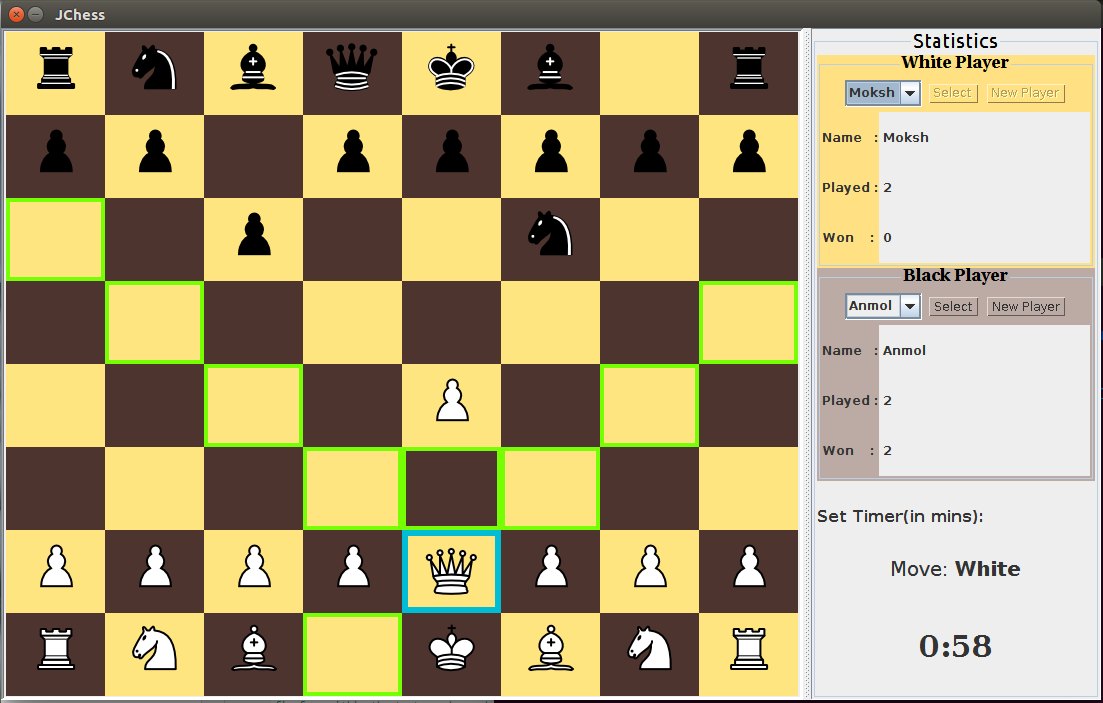
\includegraphics[scale=0.3]{SS-PossibleMoves.png} % e.g. insert ./image for image.png in the working directory, adjust scale as necessary
\caption{Possible moves being highlighted}
\label{fig:label} % insert suitable label, this is used to refer to a fig from within the text as shown above
\end{figure}

\paragraph{}
When a piece is clicked, the game obtains the possible destinations for the piece in current board configuration. These possible positions are highlighted on the board, that is, (the corresponding tiles are highlighted with a border). If the King is under check then the game filters the moves, and highlights only the moves where the king is saved from the check. If the piece is a king then the moves are filtered such that it does not move to a position where it is under a check.


\subsection{Board}
\begin{figure}[htb]
\centering
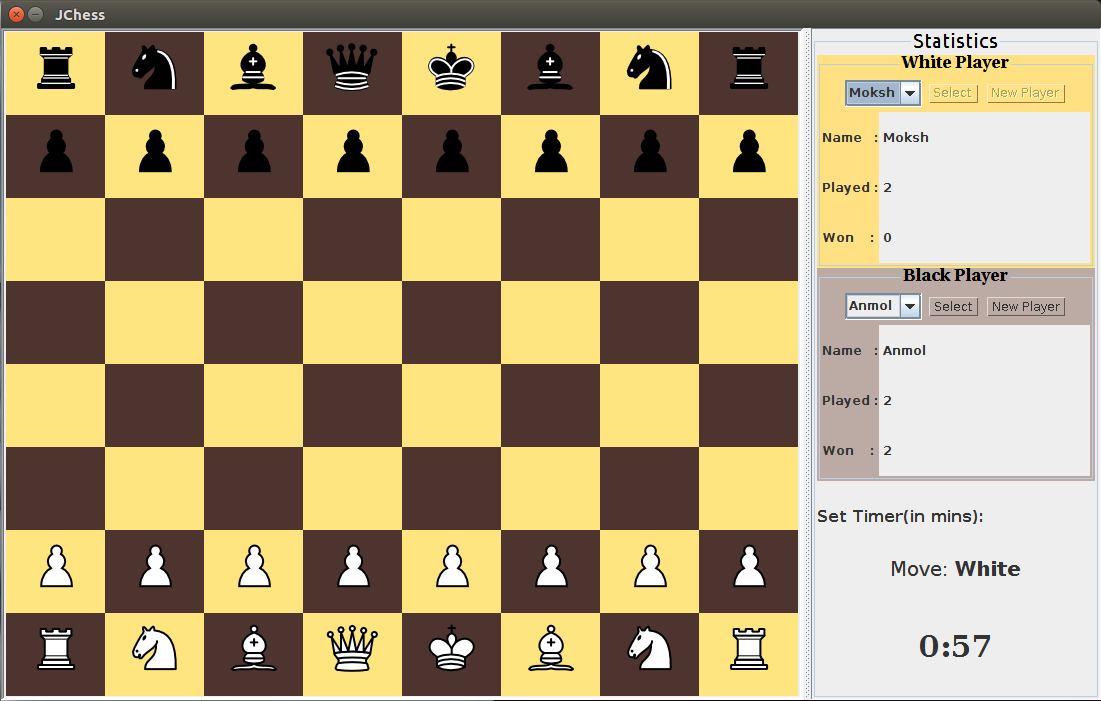
\includegraphics[scale=0.3]{SS-StartBoard.png} % e.g. insert ./image for image.png in the working directory, adjust scale as necessary
\caption{Newly created board}
\label{fig:label} % insert suitable label, this is used to refer to a fig from within the text as shown above
\end{figure}
\paragraph{}
The board consists of 64 \textit{tiles} arranged in an 8x8 grid. Each of these tiles is defined in the Tiles class. The Tile class extends extends JLabel, which is a UI Component in the Java Swing Library. Each Tile contains a reference to the piece it currently contains. The label is thus filled with the image of the corresponding piece, if any. A tile is highlighted if it is a possible destination for the current move. If the tile contains a king which is under check then it is colored red. The Tile also implements the \textit{Cloneable} Marker interface, making it easier to clone.

\subsection{Player}
\begin{figure}[htb]
\centering
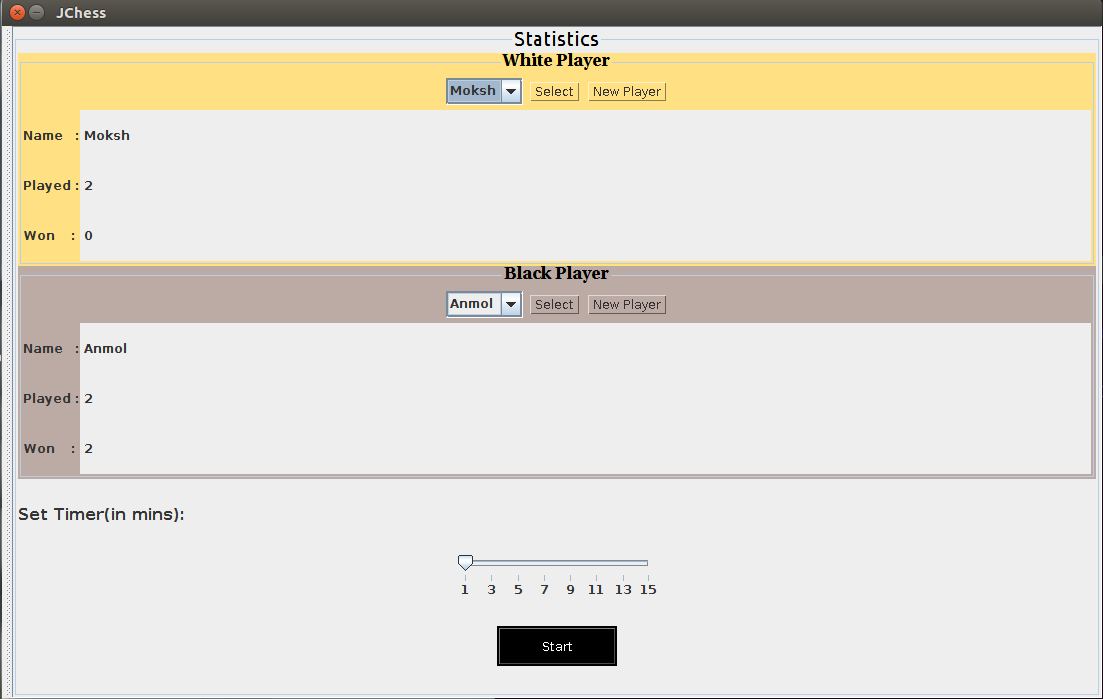
\includegraphics[scale=0.3]{SS-NewGame.png} % e.g. insert ./image for image.png in the working directory, adjust scale as necessary
\caption{User gets to select players}
\label{fig:label} % insert suitable label, this is used to refer to a fig from within the text as shown above
\end{figure}
\paragraph{}
The Player class defines the behaviour of a player in the game. It strores the name of the player, along with some other details such as games played and games won. The Player class also implements the Serializable Marker Interface to make it serializable. The Player Details are saved at the end of the game to the \textit{UserData.dat} file using the \textit{writeObject} method. When the game is started, the user can select from one of the pre-existing players stored in the game data or create a new player altogether.


\subsection{Game}
\paragraph{}
The Game class implements the main \textit{game} functionality of the the project. The Game class itself extends the JFrame class, and contains all the layouts that are displayed to the user. This includes the side panel and the board. The side panel contains the information about the Players and also displays the Timer (which can be configured at the start of the game).

\begin{figure}[htb]
\centering
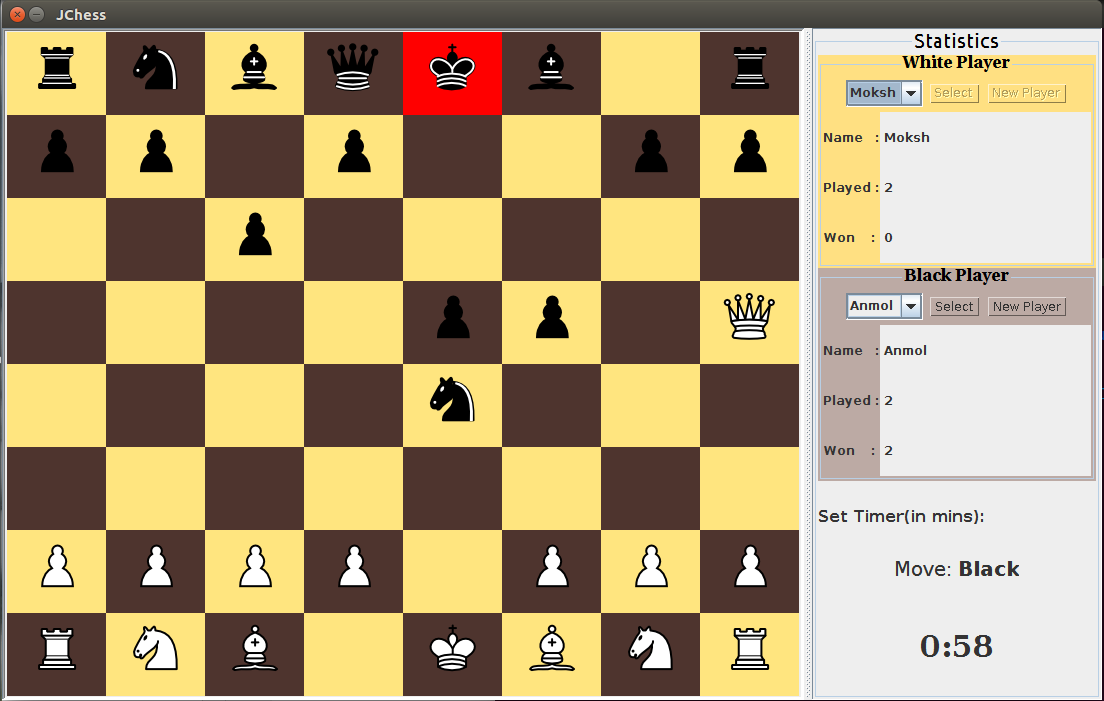
\includegraphics[scale=0.2]{SS-Check.png} % e.g. insert ./image for image.png in the working directory, adjust scale as necessary
\caption{Check}
\label{fig:label} % insert suitable label, this is used to refer to a fig from within the text as shown above
\end{figure}

\begin{figure}[htb]
\centering
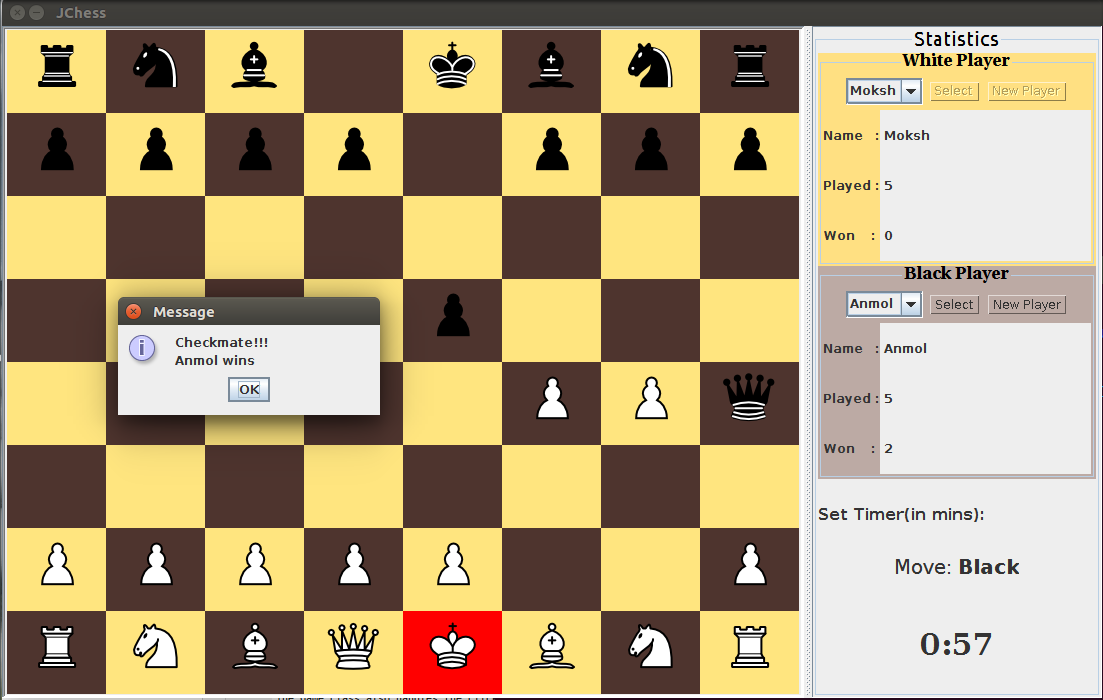
\includegraphics[scale=0.2]{SS-CheckMate.png} % e.g. insert ./image for image.png in the working directory, adjust scale as necessary
\caption{Checkmate}
\label{fig:label} % insert suitable label, this is used to refer to a fig from within the text as shown above
\end{figure}

When the game is started, the Game class is run, since it is the main class. When the game is started, the user has to select the players, and change the time limit on the timer, if required. Once the user click the \textit{Start} button, the Game class sets up the board. The Game class also handles the click event for each and appropriately highlights the possible positions and indicates if there is a check. If there is a check mate then the name of the winner is displayed and the game is restarted.

\section{Future Work}
\begin{itemize}
\item Advanced maneuvers such as castling can be implemented to make the game more function.

\item More game modes such as rapid mode can be added to make the game more versatile.

\item An AI agent can be added so the user can play against the computer in the absence of 2 players
\end{itemize}